%% The following is a directive for TeXShop to indicate the main file
%%!TEX root = diss.tex

\chapter{Introduction}
\label{ch:Introduction}

\section{Incidence and mortality of breast cancer}
Breast cancer is the most common type of cancer in Canadian women behind non-melanoma skin cancers and is the second highest cause of cancer related deaths in women. In 2020, 27,400 women will be diagnosed and 5,100 women will die from breast cancer. On average, 75 Canadian women will be diagnosed while 14 Canadian women will die from breast cancer every day. Among females, the age-standardized incidence rates (ASIR) for breast cancer rose between 1984 and the early 1990s after which it has fluctuated and the age-standardized mortality rates (ASMR) has decreased consistently for breast cancer \cite{canadian2020canadian} (\textbf{\autoref{fig:breastcancerstats}}).

\begin{figure}
\centering
\includegraphics[width=\textwidth]{Figures/chap1/breastcancerstats.png}
	\caption[Breast cancer statistics by Canadian cancer society ]
	{\small
	    \textbf{Breast cancer statistics by Canadian Cancer Society.}
	    \textbf{(a)} Percentage of all estimated new cancer cases in women in 2020.
	    \textbf{(b)} Age-standardized incidence rates (ASIRs) for selected cancers, in Canada (excluding Quebec), 1984 to2020, by sex. Shading indicates projected data.
	    \textbf{(c)} Percentage of all estimated cancer deaths in women in 2020
	     \textbf{(d)} Age-standardized mortality rates (ASMRs) for selected cancers in Canada, 1984 to 2020, by sex. Shading indicates projected data.
	}
	\label{fig:breastcancerstats}
\end{figure}

%%%%%%%%%%%%%%%%%%%%%%%%%%%%%%%%%%%%%%%%%%%%%%%%%%%%%%%%%%%%%%%%%%%%%%

\section{Breast cancer heterogeneity}
 Tumours that originate from different tissues and cells diversify in terms of their genomic as well as transcriptomic landscapes.
 However, genomic aberrations, phenotypic characteristics, such as, stromal recruitment, metastasis, evolution of drug resistance, and drug sensitivity vary between tumours that originate from the same tissue and cell type \cite{vogelstein2013cancer}. 
Tumour heterogeneity thus makes every cancer a unique disease. Heterogeneity occurs, between patients, and within patients over time and space. 
The presence of distinct subpopulations of cells within a tumour, with distinguishable genotypic and phenotypic differences, was classically demonstrated several decades ago \cite{fidler1978tumor}.
The concept of intratumour heterogeneity implies to the presence of distinct tumour cell populations (with different molecular and phenotypical profiles) within an individual tumour following variability over time during tumour growth \cite{ellsworth2017molecular, welch2016tumor}. Inter and intratumour heterogeneity have significant implications for the choice of chemotherapy to govern clinical decision-making in cancer medicine \cite{bedard2013tumour}.



\subsection{Breast cancer subtypes}
To date, several studies have shown that the breast cancer subtypes are associated with variations in treatment response and disease-specific outcomes \cite{metzger2013patterns, arvold2011age}. 
They are identified based on their histological and molecular subtypes. 
Around 50\% to 80\% of newly diagnosed breast cancer cases are
invasive ductal carcinoma (IDC) subtype, while invasive lobular carcinoma (ILC) cases make up less than 10\%. \cite{henry2019breast}.
Based on  gene expression profile studies, four clinically relevant molecular subtypes include; \textbf{Luminal A} (ER+, PR+, HER2-, Ki67low), \textbf{Luminal B} (ER+, PR-, HER2-, Ki67high or ER+, PR-/+, HER2+, Ki67low/high), \textbf{HER2+} (ER-, PR-, HER2+, Ki67high) and \textbf{Triple Negative} (ER-, PR-, HER2-, Ki67high \cite{nadia2017gm, do2020histological}.

The estrogen receptor (ER), progesterone receptor (PR), and ERBB2 also known as human epidermal growth factor receptor 2 (HER2) is routinely determined in all invasive breast carcinomas by immunohistochemistry (IHC) as recommended by cancer control committees and unions \cite{turashvili2017tumor, hammond2010college, wolff2013american}. These are categorized as subtypes of breast cancer and are characterized by their molecular profiles, morphology, and expression of specific biomarkers. The receptor status in the growing tumours also creates another complex layer of intra tumour heterogeneity. For example, some cells that express ER in breast tumours varies from 1 to 100\% cells in the tumour \cite{januvskevivciene2019heterogeneity, visvader2011cells}. These receptors are actionable targets for treatments such as hormone therapies with drugs like tamoxifen, a non-steroidal antiestrogen, used to treat estrogen receptor positive breast cancers \cite{jordan2003tamoxifen,fisher2005tamoxifen} and monoclonal antibodies, such as, herceptin that targets overexpressed ERBB2 (HER2), proven to be effective \cite{piccart2005trastuzumab,slamon2011adjuvant}.  
For the scope of this thesis, I have worked with three triple negative breast cancers (Chapter 4, 5) and one HER2+ (Chapter 4) breast cancer.

%------------------------------------------------------------
\begin{figure}
\centering
\includegraphics[width=\textwidth]{Figures/chap1/Breastcancersubtypes.png}
	\caption[Breast cancer subtypes]
	{\small
	    \textbf{Breast cancer TNBC intrinsic subtypes adapted from \cite{garrido2019insights}.}
	    \textbf{(a)} Intrinsic subtypes defined by PAM50 and PAM50 + claudin-low in The Cancer Genome Atlas (TCGA) and METABRIC data sets in \ac{TNBC}.
	    \textbf{(b)} Distribution of breast cancer subtype according to receptor status defined by IHC in TCGA and METABRIC data sets in basal-like breast cancer.
	    \textbf{(c)} Interactions among molecular classifications of TNBC based on genomic, transcriptomic, proteomic, epigenomic, and immune characterization of the tumour and its microenvironment. ER, estrogen receptor; PR, progesterone receptor; RTK, receptor tyrosine kinase; MMR, mismatch repair; CNA, copy-number alteration; AR, androgen receptor; HRD, homologous recombination deficiency; IHC, immunohistochemistry; PDJ (PD-L1/2, JAK2).
	}
	\label{fig:Breastcancersubtypes}
\end{figure}
%---------------------------------------------------------------



\begin{figure}
\centering
\includegraphics[width=\textwidth]{Figures/chap1/TNBChistologicsubtypes.png}
	\caption[TNBC histologic subtypes adapted from  \cite{bianchini2016triple} ]
	{\small
	    \textbf{TNBC histologic subtypes adapted from \cite{bianchini2016triple}.}
	    \textbf{(a)}, Histological subtypes. Some rare but relevant subtypes are shown for
illustrative purposes.
	    \textbf{(b)}, Gene-expression-based subtypes of triple-negative breast cancer (TNBC) according to PAM50 \cite{prat2013molecular}.
	    \textbf{(c)}, Gene-expression-based subtypes defined by Lehmann \textit{et al.} \cite{lehmann2011identification}
	     \textbf{(d)} Integrative clusters (IntClust) of genomic and transcriptomic data applied to basal-like breast cancer (BLBC) defined by gene-expression.
	     \textbf{(e)} Heterogeneity of tumour infiltrating lymphocytes. Tumours with low, intermediate and high lymphocyte infiltration are shown for illustrative
purposes. BL1, basal-like 1; BL2, basal-like 2; IM, immunomodulatory; LAR, luminal androgen receptor; M, mesenchymal;
MSL, mesenchymal stem-like; UNC, unclassified; UNS, unstable.
	}
	\label{fig:TNBChistologicsubtypes}
\end{figure}
%------------------------------------------------------------
\subsection{Insights into triple negative breast cancer subtypes heterogeneity}
Patient grouping defined by the absence of biomarkers ER, PR and HER2 are usually referred to as ``triple-negative breast cancers (TNBC)''. It constitutes an extremely heterogeneous group in regards to histology, genetic diversity and treatment resulting in poor prognosis. TNBC accounts closer to $\sim$~15\% in large population series of newly diagnosed breast cancers \cite{reis2008triple}.
The overall survival rate of TNBC is shorter as compared to other breast cancer subtypes and the mortality rate within the first 5 years after diagnosis is 40\%. The recurrance rate in TNBC after surgery is  around 25\% with distant metastasis developing in three years of diagnosis. Unfortunately, the median survival rate, after metastasis, is only 13.5 months \cite{dent2007triple,lin2008sites}. These incidence rates signify the need to understand the extent and mechanisms of heterogeneity in TNBC, which effects treatment outcome. 

Triple negative breast cancers have been redefined over the last decade by METABRIC consortium \cite{curtis2012genomic, dvinge2013shaping, pereira2016somatic, dawson2013new, bilal2013improving}, TCGA \cite{weinstein2013cancer}, ICGC breast \cite{international2010international} and Broad \cite{banerji2012sequence, rheinbay2017recurrent} into two major molecular sub groups (\textbf{\autoref{fig:Breastcancersubtypes} a, b}) \cite{xu2014omics}.

The first group constitutes approximately 75\% of genomically unstable sub-type, with high levels of \ac{CNA}, Loss of heterozygosity (LOH) and structural variations accompanied by basal expression pattern, ubiquitous p53-mutation and high clonal complexity \cite{shah2012clonal, garrido2019insights}. These patients have poor prognosis. The remaining around 25\%, non-basal PIK3CA-enriched TNBC, form distinct groups and have generally better prognosis. Androgen receptor (AR) expressing subset is another known subtype category of TNBC \cite{tang2012expression, rakha2007prognostic,mrklic2013expression}. There is an increasing interest in the possible efficacy of antiandrogen therapies in TNBC \cite{gerratana2018androgen,gucalp2013phase}.
All these subtypes have complex interaction between them summarized in \textbf{\autoref{fig:Breastcancersubtypes} c}.


Extensive research has focused on identifying practical subtypes of TNBC bearing uniformly actionable molecular features. They are described based on their histological and molecular classifications in \textbf{\autoref{fig:TNBChistologicsubtypes}} \cite{weigelt2009histological,bianchini2016triple}. 

\subsection{Relationship of genomic instability and heterogeneity in TNBC}
Genomic instability (GI) refers to the increased tendency to give rise to genomic alterations. It drives heterogeneity and is a hallmark of cancer and results in inter and intratumour heterogeneity \cite{hanahan2011hallmarks}.
 Cells that have intrinsic genomic instability are predisposed to increased mutation rates resulting in evolution of tumour subpopulations with remarkably distinct phenotypes such as metastatic potential and therapeutic resistance \cite{fidler1978tumor, burrell2013causes,januvskevivciene2019heterogeneity}.
TNBC show distinct patterns of copy number based genomic alterations and defects in homologous recombination (HR).
In contrast to estrogen receptor positive breast cancer, where there is a clear gain of 1q and 16p and loss of 16q and HER2 positive subtype, that shows focal high-level amplifications, TNBCs are characterized by a network of low amplitude gains and losses over short chromosome segments with many copy number transitions \cite{kwei2010genomic}.
As compared to other subtypes, TNBCs also present high levels of chromosome instability with loss or gain of larger chromosome fragments or the entire chromosome causing significant structural variation and heterogeneity \cite{lee2016mechanisms}.
The elevated genomic instability creates a complex heterogeneous tumour composed of multiple sub-clones that could progress generating clones having selective advantage conferring drug resistance. 

Genomic instability occurs through various mechanisms, including DNA damage checkpoints, the DNA repair network and the cell cycle checkpoints. BRCA-mutated TNBC are defective in homologous recombination (HR) with advanced and higher tumour grades, distinct metastasis and frequent BRCA1 mutations of $\sim$ 60\%, however, no specific association is observed for BRCA2 mutation carriers \cite{boyle2012triple, atchley2008clinical}. These mechanisms are either operated during tumour development, or influenced by external pressure including exposure to chemotherapies \cite{burrell2013causes,ding2012clonal,hunter2006hypermutation}.

These patterns of genomic instability leave distinct genetic footprints causing cancer evolution inturn affecting therapeutic outcome. 

%%%%%%%%%%%%%%%%%%%%%%%%%%%%%%%%%%%%%%%%%%%%%%%%%%%%%%%%%%%%%%%%%%%%%%

\section{Chemotherapeutic strategies in TNBC}
Due to the lack of distinct endocrine therapies and target candidates in TNBC, more traditional chemotherapy methods are employed to treat TNBC. For more than a decade, a large amount of literature has shown a significantly higher remmission rate in TNBC by using neo-adjuvant chemotherapy (NAC) \cite{liedtke2008response,symmans2017long}. Neoadjuvant chemotherapy refers to the drugs that are administered before surgery. It has been shown previously that the \ac{pCR} of platinum based alone or in combination with paclitaxel, epirubucin or doxorubicin as a neoadjuvant therapy, is between 22\% and 65\%,  
more favourable in TNBC \cite{silver2010efficacy,petrelli2014value,garber2006neo,frasci2009preoperative}. There still are many ongoing clinical trials on neoadjuvant chemotherapies selection in TNBC (including some PARP inhibitors in BRCA deficient tumours), and are reviewed in detail by Tufanno \textit{et al}. in an update article \cite{tufano2020updates}.

The adjuvant therapies are given after initial intervention, usually surgery, to achieve maximum effectiveness. The choice of adjuvant chemotherapy should be individualized based on a number of factors, including tumour stage and grade, rate of disease progression and previous chemotherapy exposure \cite{cardoso20173rd,partridge2014chemotherapy}. According to the national comprehensive cancer network guidelines, TNBCs are treated with a combination of platinum based compounds (DNA-damaging agents), taxanes (microtubule stabilizers-mitotic inhibitors), anthracyclines (DNA intercalators), cyclophosphamide (alkylating agents) and Fluorouracil (antimetabolites) \cite{daly2020nccn}.


Furthermore, most cases of TNBC have unstable genomes complicated with copy number variations, SNVs and structural rearrangements. This high degree of genomic instability can create a very heterogeneous tumour composed of multiple sub-clones which could aid in generating clones that have a selective advantage conferring drug resistance. Drug resistance, whether inherited or acquired, results in challenges to treatment and a worse outcome for the patient.

In Chapters 4 and 5, Cisplatin is selected to perturb tumours to decode clonal and evolutionary dynamics, at genomic and transcriptomic levels, respectively. To compare and contrast cisplatin induced dynamics, CX5461 (G4-quadruplex) was applied in one of the three TNBC PDX. Here we will give an overview of these two drugs.

%...............................................................

\subsection{Cisplatin}
Cis-diamine-dichloroplatinum (II) (also known as cisplatin or CDDP),  is a largely employed platinum compound that causes DNA damage in  a wide spectrum of solid cancers.  At present, around 22 clinical trials are probing the use of cisplatin to treat TNBC either as a single agent or in combination with other therapies \cite{us2017clinicaltrials}.
There is a renewed interest in treating TNBC with cisplatin.
In particular, use of cisplatin therapy has been suggested for TNBC harboring a BRCA mutation \cite{caparica2019treat,petrelli2016platinum}. 
% why there is 
%...................................................................

\subsubsection{Mechanism of action}
Cisplatin is a DNA-intercalating agent \cite{dasari2014cisplatin, kartalou2001mechanisms}. Copper transporter proteins (CTR1 and CTR2) are involved in the uptake of the cisplatin by facilitated diffusion in an inactive form \cite{arnesano2018platinum,ishida2002uptake}. Cisplatin gets activated intracellularly by a series of reactions that includes substitution of one or both cis-chloro groups with water molecules \cite{el1999reactions}. This activation takes place because of the different chloride concentration between blood plasma ($\sim${100mM}) and cell cytolasm ($\sim${4mM}) that leads to the generation of highly reactive mono- and bi-aquated cisplatin forms.


%-------------------------------------------------------------------
\begin{figure}
\centering
\includegraphics[width=\textwidth]{Figures/chap1/CisplatinMA.png}
	\caption[Mechanism of action of cisplatin]
	{\small
	    \textbf{Mechanism of action of cisplatin modified from \cite{galluzzi2012molecular}}.
	     Intra cellular cisplatin is rapidly aquated due to reduced cytoplasmic concentration of chloride ions. Aquated cisplatin binds to nuclear DNA, thereby promoting DNA damage response. In the cytoplasm, interact with several nucleophiles, including mtDNA as well as multiple mitochondrial and extracellular proteins causing formation of oxidative and reticular stress; provoking a signal transduction cascade that involves pro-apoptotic,BID, BCL-2 family members, as well as VDAC1 and activation of TP53 leading to MOMP and cell death.
	    TP53 activation could directly lead to Cell senescence not shown in the figure. MOMP, mitochondrial outer memberance permeabilization;BID, Bax-like BH3 protein; VDAC, Voltage-dependent anion channel; mtDNA, mitochondrial DNA.
	}
	\label{fig:CisplatinMA}
\end{figure}
%-----------------------------------------------------

The platinum atoms of cisplatin cross-links DNA by making covalent bonds with purine bases in particular with nucleophilic N7 sites. Homotypic intra stand and low percentage of inter strand cross-links result in the generation of DNA-adducts that interfere with DNA replication and RNA transcription. If DNA is not repaired, DNA-damage induced cell-cycle arrest either becomes permanent (an oncosupressive response called senescence) or mitochondrial apoptosis is triggered \cite{fichtinger1985adducts, rabik2007molecular,lopez2013hallmarks}. 

%This effectiveness seems to be due to the unique properties of cisplatin, which enters cells via multiple pathways and forms multiple different DNA-platinum adducts while initiating a cellular self-defense system by activating or silencing a variety of different genes, resulting in genetic and/or epigenetic alterations.
The main signaling cascade that links cisplatin induced DNA lesions to apoptosis involves sequential activation of ATM and RAD3 related protein (ATR, a sensor of DNA damage) and checkpoint kinase 1 (CHEK1, is the downstream effector of ATR) that  eventually phosphorylates the tumour suppressor protein TP53 at serine 20    \textbf{(\autoref{fig:CisplatinMA})} \cite{shieh2000human, cimprich2008atr}. Activated TP53 promotes mitochondrial outer membrane permeabilization (MOMP).  MOMP alone or with stimulatory signals via pro-apoptotic BCL-2 family (BID, BAK1, BAX) \cite {tajeddine2008hierarchical} sets off the caspase dependent cascade and some independent mechanisms that lead to cell death. Checkpoint kinase 2 (CHEK2, is the downstream target of ATM), along with induced cell cycle arrest  (not cell death) through ATM signaling, also responds to cisplatin in an ATM-independent fashion \cite{pabla2008atr}. 

In the cytoplasm, the interaction of cisplatin with glutathione (GSH), metallothionines or mitochondrial proteins for example, voltage-dependent anion channel (VDAC), derives the generation of reactive oxygen species (ROS). ROS and nitric oxide (NO) exacerbate cisplatin toxicity along with increasing the opening of permeability transition pore complex (PTPC) on mitochondria \cite{godoy2012endogenously}. There are also evidence in literature that CHEK1 activates MAPK pathway signaling, mediated by extracellular signal-regulated kinases, c-JUN N-terminal kinases and stress-activated protein \cite{persons2000effect, yeh2002increase}.

\subsubsection{Mechanism of cisplatin resistance}
Cisplatin resistance can arise from transformation in the processes that precede the binding of cisplatin to its actual targets, including cytoplasmic structures and DNA. These factors are categorized as \textbf{pre-target resistance} \textbf{(\autoref{tab:pretargetcisplatinresistance})}. Briefly, copper transporter 1 (CTR1) mediate major fraction of cisplatin intake \cite{more2010role,ishida2010enhancing, holzer2006contribution}, whereas ATPase, copper transporting, beta polypeptide (ATP7B), is involved in cisplatin export \cite{katano2002acquisition,komatsu2000copper, aida2005expression}. Some plasma membrane transporters have been proposed to contribute to the extrusion of cisplatin, including ATP-binding cassette, subfamily C member 2, best known as multidrug  resistance-associated protein 2 (MRP2) \cite {cui1999drug,korita2010multidrug,liedert2003overexpression} and ATP-ase, class VI, type IIB (ATP11B) \cite{moreno2013atp11b}. Moreover, cisplatin resistant cells also exhibit high levels of metallothioneins \cite{kelley1988overexpression,kasahara1991metallothionein} and GSH, an enzyme that catalyzes GSH synthesis (i.e., gamma glutamylcysteine synthetase) and conjugates with cisplatin \cite{lewis1988glutathione,chen2010role}. 

%----------------------------------------------------------------------
\begin{table}[htbp]
   \centering
   \caption{Pre-target cisplatin resistance factors. Modified from \cite{galluzzi2012molecular}}
\begin{tabular}{p{1.5cm}p{5cm}p{5cm}p{1cm}}
\hline
\textbf{Genes/ Factors} & \multicolumn{1}{l}{ \textbf{Mode of Action}} & \multicolumn{1}{p{5cm}}{ \textbf{Importance}} & \multicolumn{1}{p{5cm}}{ \textbf{References}} \\ \hline

CTR1   & Reduced uptake, Plasma membrane copper transporter & Downregulated in resistant cells. CTR1 depletion increases cisplatin resistance. Copper chelators enhance the uptake and efficacy of cisplatin & \multicolumn{1}{p{5cm}}{ \cite{more2010role, ishida2010enhancing,holzer2006contribution,katano2002acquisition}} \\

ATP7A/ ATP7B & Increased efflux, Copper-extruding P-type ATPases involved in the regulation of ion homeostasis & Upregulated in cisplatin-resistant cells. ATP7B expression levels may predict the efficacy of cisplatin chemotherapy.  & \multicolumn{1}{p{5cm}}{\cite{katano2002acquisition,komatsu2000copper,nakayama2002copper,safaei2004role,aida2005expression}} \\ 

MRP2   & Increased efflux, Member of the ABC family of plasma membrane transporters. Mediates the ATP-dependent cellular efflux of cisplatin. & Overexpressed in cisplatin-resistant cells. Modulation by antisense cDNA enhances cisplatin sensitivity. Expression levels affect the efficacy of cisplatin regimens. & \multicolumn{1}{p{5cm}}{\cite{cui1999drug,korita2010multidrug,liedert2003overexpression, yamasaki2011role}} \\

GSH/ GCS/ GST & Increased inactivation, GSH scavenges electrophiles and ROS. GCS catalyzes GSH synthesis. GST conjugates GSH to cisplatin and facilitates its extrusion. & Resistant cells often exhibit high levels of GSH, GCS and GST.  & \multicolumn{1}{p{5cm}}{\cite{lewis1988glutathione,chen2010role}} \\

Metallo-thionein & Increased inactivation, Intracellular thiol-containing proteins involved in the detoxification of metal ions. & May bind and inactivate cisplatin.  & \multicolumn{1}{p{5cm}}{\cite{kelley1988overexpression,kasahara1991metallothionein}} \\   \hline
\end{tabular}%
\begin{tablenotes}
\small
      \item  {CTR1,copper transporter receptor 1; MRP, multi-drug resitance proteins; ROS, reactive oxygen species; GSH, glutathione; GCS,gamma-glutamylcysteine synthetase; GST, glutathione S-transferases}.
    \end{tablenotes}
 
   \label{tab:pretargetcisplatinresistance}%
 \end{table}%
%-----------------------------------------------------------------------

The mechanism of \textbf{on-target cisplatin resistance} is believed to arise in particular with the removal of cisplatin DNA-adducts and subsequent apoptosis can be defective in cisplatin-resistant cancer cells due to a variety of mechanisms including nucleotide excision repair (NER) proficiency \cite{wood2000dna, shuck2008eukaryotic}. They are summarized in \textbf{\autoref{tab:ontarget}}. In addition, another proposed mechanism for cisplatin resistance involves high expression of the high-mobility group box protein 1 (HMGB1), that appears to bind selectively to cisplatin DNA crosslinks and interferes with \ac{NER} while HMGB3 is associated with the promoter regions of ATR and CHK1 \cite{awuah2017repair, mukherjee2019targeting}. 


%------------------------------------------------------------

\begin{table}[htbp]
   \centering
   \caption{On-target cisplatin resistance factors. Modified from \cite{galluzzi2012molecular}}
    \begin{tabular}{p{1.5cm}p{5cm}p{5cm}p{1cm}}
     \hline
      \textbf{Genes/ Factors} & \multicolumn{1}{l}{ \textbf{Mode of Action}} & \multicolumn{1}{p{5cm}}{ \textbf{Importance}} & \multicolumn{1}{p{5cm}}{ \textbf{References}} \\ \hline
ERCC1  & Increased NER proficiency, Single-strand endonuclease, in association with ERCC4/XPF incises DNA on the 5' side of cisplatin adducts. & ERCC1 expression negatively correlates with  cisplatin clinical responses in multiple human cancers & \multicolumn{1}{p{5cm}}{\cite{dabholkar1992ercc1, metzger1998ercc1, bellmunt2007gene, shirota2001ercc1}} \\
MLH1 & MMR deficiency, Component of a multiprotein complex that excides and repairs DNA mismatches. Implicated in DNA damage signaling and apoptosis. & MLH1 deficiency is sometimes associated with  cisplatin resistance (and increased TLS).  & \multicolumn{1}{p{5cm}}{\cite{aebi1996loss, gifford2004acquisition}} \\
MSH2  & Forms heterodimers that detect DNA lesions including base-base mismatches. & Low MSH2 levels predict  cisplatin benefits in patients with resected lung cancer. & \multicolumn{1}{p{5cm}}{\cite{kamal2010muts}} \\
POLH & Increased TLS, DNA polymerase that substitutes stalled replicative polymerases and includes nucleotides opposite to the DNA lesion. & POLH upregulation correlates with short patient survival. & \multicolumn{1}{p{5cm}}{\cite{alt2007bypass, shachar2009two}} \\
REV3/ REV7 & Catalytic (REV3) and structural (REV7) subunits of the TLS DNA polymerase . & REV3 defects correlate with increased cisplatin sensitivity in cancer cell lines. REV overexpression is associated with  cisplatin resistance  & \multicolumn{1}{p{5cm}}{\cite{wittschieben2006loss, roos2009translesion}} \\  
BRCA1/ BRCA2 & Increased HR proficiency, HR DNA repair. Regulation of transcription and cell cycle progression. & BRCA1/2-deficient tumours respond better to  cisplatin. Secondary mutations that restore BRCA function favor acquired chemoresistance.& \multicolumn{1}{p{5cm}}{\cite{narod2004brca1, edwards2008resistance, sakai2008secondary}}  \\  
VDAC & Cisplatin binding proteins, protein of the OM that mediates vital functions but also participates into the PTPC.& Depletion/or inhibition of VDAC increases  cisplatin resistance. Might also be involved in post-target resistance.& \multicolumn{1}{p{5cm}} {\cite{yang2006cisplatin,kroemer2010autophagy,tajeddine2008hierarchical}}\\  
    \hline
     \end{tabular}%
  \begin{tablenotes}
      \small
      \item  {ERCC1, excision repair cross-complementing rodent repair deficiency, complement group1, HR, homologous recombination; TLS, translesion synthesis; OM, mitochondrial outer membrane; XPF, xeroderma pigmentosum complementation group; VDAC, voltage dependent anion channel; PTPC, permeability transition pore complex.}
    \end{tablenotes}
 
   \label{tab:ontarget}%
 \end{table}%

%------------------------------------------------------------------------

\begin{figure}
\centering
\includegraphics[width=\textwidth]{Figures/chap1/circumventingcisplatinresistance.pdf}
	\caption[Mechanism of action of cisplatin]
	{\small
	    \textbf{Inhibition strategies at various levels of cisplatin resistance mechanisms. Modified from  \cite{galluzzi2012molecular}}.
	     Cisplatin resistance most often has a multifactorial nature, implying that targeting one mechanism of resistance at a time has very low chances to result in significant chemosensitization. Thus, combination strategies for blocking cisplatin resistance at multiple levels should be designed. With regard to this, detailed information on the patient genetic and epigenetic background might be critical for determining which specific mechanisms should be targeted to fully circumvent chemoresistance. CTR, Copper transporter receptor; EGFR, epidermal growth factor receptor; HSP, heat-shock protein; PTEN, phosphatase and tensin homolog; TLS, translesion synthesis.
	}
	\label{fig:circumventingcisplatinresistance}
\end{figure}

%----------------------------------------------------------------------

\textbf{Post-target resistance} to cisplatin can result from alterations in signal transduction pathways that mediate apoptosis in response to DNA damage. Non-repairable cisplatin-induced DNA damage leads to the activation of a multi-branched signaling cascade with proapoptotic outcomes. Several groups have provided evidence that predominant mechanisms involves the inactivation of \textit{Tp53}, which exists in around half of all human cancers \cite{kirsch1998tumor}. Reportedly patients harboring wild-type \textit{Tp53} have a higher probability to take advantage from cisplatin as compared to the patients with \textit{Tp53} mutations \cite{vousden2007p53,gadducci2002molecular}. 
Furthermore, inhibition of PDGFR$\beta$ mediated phosphorylation of AKT by Ly294002 reversed cisplatin resistance \cite{juliachs2014pdgfrbeta}. Somatic mutations within PI3KCA, AKT and FGFR3 were also reported in cisplatin resistance \cite{feldman2014presence}. Pre-clinical studies indicate that targeting PDGFR/PI3K/AKT pathway may reverse cisplatin resistance \cite{juliachs2013effectivity}.
Upregulation of IGF1R expression and signaling was also found to contribute to acquired cisplatin resistance \cite{selfe2018igf1r}. 

Variations in any of the factors that regulate and carry out apoptosis have the potential to influence cisplatin sensitivity. It could be triggered by DNA damage or oxidative stress via the mitochondrial pathway. Numerous proteins including death receptors, cytoplasmic adaptors. pro- and antiapoptotic members of the BCL-2 family, caspases, calpains and many others \cite{jain2011molecular, janson2010resistance, michaud2009bcl}. Ryan \textit{et al.} reported that BIRC5 (Survivin) overexpression is associated with chemoresistance and poor prognosis in multiple types of cancer \cite{ryan2009survivin}. 

Cisplatin-resistant phenotype can also be sustained through \textbf{off-target resistance} including the alterations in signaling pathways that are not directly engaged by cisplatin. Relavant factors include are autophagy, which is evolutionary conserved response to stress conditions including chemotherapy \cite{tan2019trp14}, DYRK1B is a conserved tyrosine kinase that is usually overexpressed in breast cancers and mediates antiapoptotic effects.  \cite{hu2010depleting}, ERBB2 \cite{fijolek2006p53}, HSP (heat shock proteins)  are chaperones that exert prosurvival functions in response to a variety of stress conditions including cisplatin \cite{ren2008down}. 
%and TMEM205 \cite{shen2010elevated}.

In summary, there are at least four distinct but broad categories of mechanisms by which cancer cells become resistant to cisplatin. The major hurdle to overcome this clinically relevant issue is that often more than one resistance mechanism is activated thus exhibiting a multifactorial consequences of cisplatin resistance. It has been speculated that at least two mechanisms should be targeted to restore cisplatin sensitivity, for example, combined interventions that could inhibit pre-target resistance (such as, copper chelators and prooxidants) and/or inhibition of post, on  or off target mechanisms (such as translesion synthesis (TLS) inhibition PI3K/AKT1 inhibition or blockers of autophagy)  \textbf{(\autoref{fig:circumventingcisplatinresistance})} may possibly restore cisplatin sensitivity. It is hard to decide which pathways should be targeted and what combination strategies should be applied to overcome resistance because all mechanisms are not operated at the same time as we observed in chapter 5 while tracking changes in pathways over drug exposure and depends on duration of drug exposure and type of tumour expressing proteins and pathways.

\subsection{CX5461: G4 stabilizer} 
CX5461 is a small molecule G-quadruplex stabilizing compound. It was developed as a selective RNA polymerase I inhibitor \cite{drygin2011targeting}. Recent evidence suggests that it causes DNA damage and induces selective lethality in BRCA1/2 deficient tumours \cite{xu2017cx}, resulting in a first in human Canadian clinical trial (CCTG-IND231). 
 
 \subsubsection{G-quadruplex structures}
G-quadruplex (G4) structures arise transiently at guanine-rich sequences in the folded DNA and RNA, when two or more G-tetrads stack on top of each other and coordinate monovalent cations, such as K+ and Na+ \cite{sen1990sodium} \textbf{(\autoref{fig:G4structures} a)}. Each tetrad is composed of four G residues that are linked by the sugar-phosphate backbone and connected through Hoogsteen-type hydrogen bonds \cite{kwok2017g}. G-quadruplex structures can fold intramolecularly from a single G-rich strand, or intermolecularly through dimerization or tetramerization of separate filaments. They both can present prarallel or anti parallel topologies \textbf{\autoref{fig:G4structures} b}. The length of loop can vary (1-7 nucleotides), with smaller loops being more stable\cite{huppert2010structure}.
G4 sequences mainly clustered in central genomic regions, namely single-stranded 3' overhangs in telomeres, gene promoters, especially oncogenes and DNA replication origins. In cancer cells these structures are important in DNA replication, telomere maintenance, and regulation of transcription and translation \textbf{\autoref{fig:G4structures} c, d, e} \cite{rhodes2015g, maizels2013g4}. Literature based on large scale DNA sequencing on human genome have revealed over 700,000 putative G4 sites and 10,000 of them have been identified from ChIP-seq using an antibody that recognises G4 structures \cite{siddiqui2002direct, granotier2005preferential, chambers2015high, hansel2016g}.

%--------------------------------------------------------------------------
 \begin{figure}
\centering
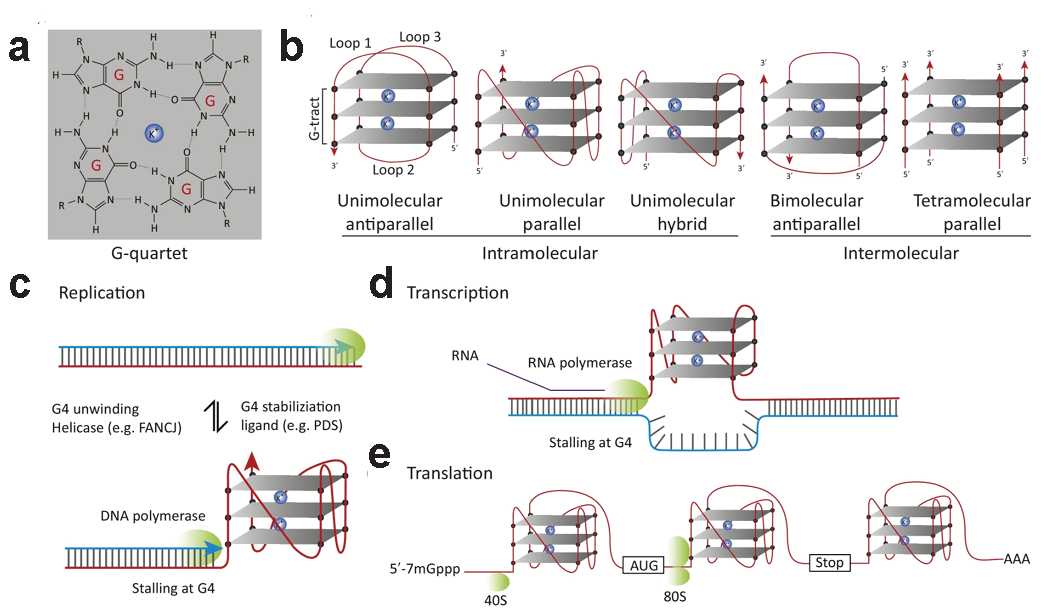
\includegraphics[width=\textwidth]{Figures/chap1/G4structures.png}
	\caption[The G4 structures and their biology]
	{\small
	    \textbf{The G4 structures and Biology. Modified from \cite{kwok2017g}}.
	   \textbf{(a)} Chemical structure of a G-quartet. Potassium ion (K+) sits within the G-quartets for stabilization. G-quartets stack on each other to form G-quadruplex \textbf{(b)} Representative topologies of G-quadruplex structures. \textbf{(c-e)} Representative G-quadruplex-associated biology: regulation of \textbf{(c)} DNA replication, \textbf{(d)} transcription, and \textbf{(e)} translation
	}
	\label{fig:G4structures}
\end{figure}
%------------------------------------------------------------------------------ 
 
 \subsubsection{CX5461 leads to synthetic lethality with  DNA repair pathways deficiency}
 The dominant feature of the p53/basal expression group of TNBC is genomic instability \cite{yu2013identification}. It is important to identify specific subgroups that could be targeted through synthetic lethal approaches, analogous to PARP inhibitors that exploit loss of homologous recombination (HR) repair  \cite{fong2009inhibition}.
 CX5461, in addition to polymerase 1 inhibition and G4 stabilization, has been recently shown to have activity in \ac{HR} and \ac{NHEJ} deficient cancer cells \cite{zimmer2016targeting,xu2017cx}. 
 BRCA1/2 deficiency leads to compromised HR repair, generating an increased error-prone DNA repair and ultimately, genomic instability. The BRCA2/RAD51 complex is also involved in many other aspects of genome instability, such as stalled DNA replication fork stabilization \cite{schlacher2011double}, R-loop resolution \cite{bhatia2014brca2} and repairing G-quadruplex (G4) associated DNA damage.
 Studies have shown that stabilization of G-quadruplex forming regions of the genome results in synthetic lethality in DNA repair deficient cancers including HRD, non-homologous end joining (NHEJ) \cite{xu2017cx, mcluckie2013g, zimmer2016targeting}. 
  
We also reported that both CX5461 and the related compound CX3543 induce DNA damage and are dependent on BRCA1/2-mediated HR and DNA-PK-mediated NHEJ pathway for damage repair \cite{xu2017cx}.

%%%%%%%%%%%%%%%%%%%%%%%%%%%%%%%%%%%%%%%%%%%%%%%%%%%%%%%%%%%%%%%%%

\section{Clonal theory of cancers and relationship to population genetics.}
The notion of clonal structure and its emergence in cancers was synthesized and summarized several decades ago by Peter Nowell, from many prior observations of chromosomal heterogeneity during tumour evolution \cite{nowell1976clonal}. The central idea is that cell division and mutation give rise to heritable marks which can be used to identify the relationships between cells. Many generations of cell division, mutation and selection give rise to a highly heterogeneous tumour composed of different groups of genotypes. Each group is characterized by a defined heritable marks, including mutations that affect a single base to copy-number aberrations affecting large genomic regions. Thus, a clone is defined as a group of cells related to each other by descent through a unitary origin. 

By \textbf{identifying and studying the properties of clonal subpopulations}, the dynamics of cancer over time and under selective pressures of treatment and metastasis can be understood \cite{aparicio2013implications}. This implies presence of multiple genotypically and/or phenotypically distinct cell subpopulations within a single growing tumour.

The terms \textbf{clonal dynamics and clonal evolution} should not be confused. The change in clone-size and number of cells within a clone is known as dynamics, while evolution is the appearance of new clonal genotypes (by mutations, change in copy number or epigentic state changes) in a growing tumour populations. 
Clonal dynamics within a tumour can be complicated as the clonal population may change in response to drug exposure or any other external pressure over time.

The concepts of clonal theory, phylogenetics, evolutionary population genomics and single cell biology are now converging.


\subsection{Identifying clonal structure and their relationships}

Any measurable heritable sequence variant from the genome such as single nucleotide variant (SNV) or copy number (CN) can be used to define clonal structure. 
Other include some epigenetic marks, eg. DNA methylation and transcriptional states or to insert a random viral barcode labelling of single cells where the cellular dynamics in question are not tightly linked to genomic variation. These approaches could be combined. However, in this dissertation we have used copy number as a heritable mark to define a clonal structure. Copy number alterations are important in breast cancer \cite{zhang2009copy, pollack2002microarray}
that has been understudied as a source of clonal genotypes. This is relevant, because as in chapter 5, CNA have a direct influence on gene transcription over many genes, thus the genotypes may also have deterministic significance. \textbf{Clonal genotype} is defined as the set of mutations, SNV or CNA uniquely defines membership of the clone. Advances in single-cell genomics are widely used to directly infer clonal genotypes \cite{macosko2015highly,laks2019clonal}. 

 \textbf{Clonal lineage relationship} is defined by the ordinal relationship between the clones over time. These relationships are considered as branched, treelike structures. However, defining a sub population from SNV or CNV information and computing a phylogeny, describes hierarchical ordering. Phylogeny shows a relationship between the cells to the lineage identified cell population as described in subsections below:
 %----------------------------------------------------------------
 
 \begin{figure}
\centering
\includegraphics[width=\textwidth]{Figures/chap1/phylogenetictree.png}
	\caption[Diagram of a phylogenetic tree]
	{\small
	    \textbf{Diagram of a phylogenetic tree}.
	 The top red node represents the ancestral node which in rooted phylogentic tree gives rise to new clones in evolving cancer.  Blue dotted circles show major cuts with big clades while red dotted circles show independent small clades. First, left emerging line shows cut in the tree giving rise to monophyletic branch with clone A and B. On right, cut leads to a major clade mentioned as clade 2. Under this major clade more smaller cuts in the phylogenetic tree gives rise to smaller clades that forms polyphyletic tree. Blue dotted circles show major cuts with big clades while red dotted circles show independent small clades.
	}
	\label{fig:phylogentictree}
\end{figure}
 \subsubsection{Phylogenetic representation of clonal evolution and clonal relationship}
Cancers are understood to evolve by mutation of the genome. Decoding cancer evolution approach is essential to understand how therapeutics and progression work, which requires phylogenetics \cite{burrell2013causes, tabassum2015tumorigenesis}. 

The phylogeny of a tumour gives insights into the sequence of events that occurred during tumour evolution but the main challenge is to resolve the subpopulation structure of a heterogeneous tumour sample. Developments in cancer evolution studies and advanced single cell technologies \cite{laks2019clonal} have further  stimulated development of new phlyogenetic methods, building on a rich literature from classical studies of heredity and evolutionary genomics \cite{schwartz2017evolution}. 

A Phylogenetic tree is a diagram that depicts the cell division and inheritance as a branching process whose leaves represent the genotypes observed at the present time and whose internal nodes inferred ancestral genotypes \cite{satas2020scarlet}.
It is useful for organizing the clonal genotypes based on their heritable marks. Tumour cells sharing the same heritable marks, such as, SNV (single nucleotide variation) or CNV (copy number variation), can be grouped into one clone that form the terminal ends of tree. Then, clonal lineage is identified by placing cells with distinct genotypes on the tree branches based on their relationship to each other (using tree cutting methods). A clade represent a part of a tree that includes an ancestral lineage and all the descendants of that ancestor which can be referred to as monophyletic or polyphyletic.  A monophyletic clade can be separated from the root with a single cut, whereas a polyphyletic group needs two or more cuts \textbf{(\autoref{fig:phylogentictree})}. Clones in the same clade share a portion of history that is common to all members of the same clade and different from the clones in other clades \cite{baum2008reading, baum2008phylogenics}.

Certain assumptions are made in the calculation of phylogenetic trees, especially with respect to the appearance and stability of new and existing genotypes over time.
Perfect phylogeny is a term used in computational phylogenetics to denote a phylogenetic tree in which all internal nodes are labeled such that all events (SNV or CNV) evolve down the tree without homoplasy (gain or loss occurring independently in separate lineages over the course of evolution) \cite{gusfield1997algorithms}. Conceptually, the perfect phylogeny model is based on the \textbf{infinite sites} assumption, developed for and largely applicable to single base mutations (SNV), that there are an infinite number of sites  where events can occur. Every new event can occur only once in the whole tree at a novel site and there would be no homoplasy or back mutation. In this model, for example, copy number are gained with low probability (0 to 1 only once), but that are lost with much higher probability (1 to 0 without constraint).

Persistent phylogeny, is an extension of perfect-phylogeny, in which a trait (SNV or CNV) can only be gained once (0 to 1) on the tree, but differs to it in that it allows the trait (SNV or CNV) to be lost exactly once (1 to 0).

In the calculation of phylogenetic trees, \textbf{optimality criteria} are used to determine how closely an inferred tree adheres to the assumptions of the phylogeny:
%\textbf{Optimality criterion} include assumptions that allowed to state that the inferred tree is close to the reality.

\textbf{(a)} Parsimony methods identify the phylogeny that requires the fewest necessary changes to explain the differences amongst observed sequences (the smallest number of steps needed to explain the data). They are considered as model free simplest procedure that imposes minimum restrictions upon permitted event changes. Free reversibility of events is allowed.

\textbf{(b)} Maximum likelihood evaluates evolutionary history in terms of the probabilities of sequences that a proposed model of an evolutionary history with higher probability of giving rise to the observed data is preferred to one with lower probability. 

%\textbf{(ii) Algorithmic methods:} Hierarchical cluster analysis (UPGMA-unweighted pair group method with arithmetic mean) and Neighbour joining:
%These methods estimate a phylogenetic tree by defining a specific sequence of steps that leads to the determination of a tree.

In this dissertation, for the sake of extracting meaningful knowledge from the timeseries data and to understand cancer evolutionary forces acting on clones, we applied a cluster type phylogenetic model that is based on perfect phylogeny and taking presence and absence of changes in the copy number profiles. 
Cluster analysis is different from neighbor joining in that it refers to the ultrametric properties of the tree that includes:

 \textbf{(a)} Branch distance between two taxa is equal to the sum of branches joining them.

\textbf{(b)} Tree is rooted so that all taxa clades are equidistance from the root. The root (usually unlabelled) corresponds to the common ancestor of all clones.

\textbf{(c)} Clock assumptions, that changes occur at the same rate in all lineages at any given time.

Another important concept in phylogenetics is \textbf{phylogenetic distance or branch length} which explains the number of events that are required to go from one node to another. Clock type branch length is important to understand cancer evolution because its important to know at what rates the events are occurring. The phylogenetic model used does not measure clock like rates as these are not understood for CNA and so phylogenetic distance is based on the number of discrete events.

\textbf{Cancer cells can violate the rules of perfect phylogeny.}
The assumptions of perfect phylogeny or persistent perfect phylogeny are more likely to be violated in the data explored in this dissertation. This is because the model of \texttt{sitka} \cite{dorri2020efficient} uses 
 CNA-change points, i.e. markers (breakpoints) instead of integer CNA states as phylogenetic traits. 
While using \textbf{breakpoints (points of copy number change)} as phylogenetic perfect persistence phylogeny model, non-overlapping CNA events do not violate the phylogeny assumptions, but the overlapping events could cause violation by two scenarios in cancer cells:

\textbf{- There could be a copy number gain from an ancestral cell followed  by an overlapping loss event}. This happens in cancers quite often as if chromosome is gained, it could be lost but in perfect phylogeny, \textbf{back mutations} are not allowed. The second loss event would mask or remove the end point of the first event.

\textbf{- There could be a copy number loss followed by an overlapping copy loss}. In cancers, the second overlapping loss event does happen on the same copy as the first. 
All the change in copy number (breakpoints) could occur independently in any lineages which goes against the rule of perfect phylogeny which assumes all events evolve down without homoplasy.  

 \textbf{\texttt{sitka}} (new method of building a phylogeny) assumptions are made to get simplified phylogenetic tree similar to perfect persistence phylogeny, although, the single cancer cell DNA sequencing data could also violate its assumptions:

\textbf{1. There is a change point without noise.} In \texttt{sitka} binary values, 0 and 1 are considered as loss and gain respectively. Violations occur as actually binary values are not observed. Incorrect change point estimates (as a result of noisy HMM CNV calls). 
Markers inconsistent with perfect phylogeny assumptions can be accounted as noise. A complication of parameterizing copy number segments in the genome only with breakpoints, is that a single event could be a small deletion or an entire chromosome. This complicates the interpretation of potential phenotypic impact of genotypes. 


\textbf{2. Infinite site assumptions.} Many infinite events are occurring. Phylogenetic trait arises exactly once on rooted tree topology and all individual cells descending from that position will inherit that trait.
CNV typically occurs at different loci but because of the binning of the data, it could be possible to see two events in the same bin as explained above.

\textbf{3. Considers exact one gain and one loss (perfect persistence phylogeny).} In cancer evolution this scenario doesn't happen as such as explained above, causing the violation.



 
 
 
 %is simplified to the breakpoints of copy number segments. the actual copy number state is not encoded.
 %we are defining clones based on their copy number profiles by using \texttt{sitka (see methods)}, which uses type of perfect phylogeny with same assumptions.

% However,in molecular evolution, if the method of tree construction is measuring single changes of amino acid or a single nucleotide variant (SNV), it could be easy to interpret but if the tree building model is taking CNA as an event then branch length becomes more important.

 Taking change in copy number as an event is more complicated because that single event could be a small deletion or it could be a whole chromosome loss/gain, which in turn has implications in cancer biology. We know that in case of copy number, chromosomal gain can occur independently, which is against the model because it does not allow homoplasy.

If a chromosome is lost, it cannot be regained but if we gain a chromosome, it could be lost, meaning back mutation is possible. Also, it is plausible that events can occur more than once in cancer cells, for example, chromosomal missegregation can occur in mitosis. In this dissertation, we are using the state of gaining a chromosome to mean a genotype, so that could have occurred independently more than once because of the nature of the data itself.

  
%Developments in cancer evolution studies and advanced single cell technologies have further stimulated development of new phlyogenetic methods, building on a rich literature from classical studies of heredity and evolutionary genomics \cite{schwartz2017evolution}.

%A Phylogenetic tree is a diagram that represents the underlying branching process and cell divisions whose leaves represent the cells observed at the present time and whose internal nodes inferred ancestral genotypes \cite{satas2020scarlet}.
%It is useful for organizing the clones based on their heritable marks. 

%Quantification of intra-tumor heterogeneity and evolutionary tree construction plays a role in diagnosis and treatment \cite{burrell2013causes, tabassum2015tumorigenesis}. It provides insights into the sequence of events that occurred during tumor evolution.

%Standard algorithms have been used by majority of studies of tumour phylogenetics that were developed for species phylogenetics (for example, maximum parsimony, minimum evolution, neighbour joining,  UPGMA (unweighted pair group method with arithmetic mean), or various maximum likelihood or Bayesian probabilistic inference methods \cite{de2014spatial, zhang2014intratumor, brocks2014intratumor, navin2011tumour, xu2012single, huelsenbeck2001bayesian, felsenstein2004inferring}. Recent developments in the filed has modified algorithms that are taking into account the specifics to tumor evolution \cite{chowdhury2013phylogenetic, yuan2015bitphylogeny, jahn2016tree}.

%Quantifying intra-tumor heterogeneity and reconstructing the evolutionary history of tumor cells is critical for the diagnosis and treatment \cite{burrell2013causes, tabassum2015tumorigenesis}. Tumor evolution  is typically described by a phylogenetic tree (phylogeny), whose leaves represent the cells observed at the present time and whose internal nodes represent ancestral cells \cite{satas2020scarlet}.
%The phylogeny methods are established on defining certain traits or inherited marks on observed individual cells. The majority of single cell phylogenetic tree inferences focus on point mutations \cite{singer2018single, zafar2017sifit, schwartz2017evolution}. Others markers include \ac{SNV} \cite{bashashati2013distinct}, \ac{CNVs} \cite{navin2011tumour}, DNA methylation, histone marks or RNA expression \cite {brocks2014intratumor, yates2012evolution, greaves2012clonal}.

%Distance based and agglomerative clustering methods such as neighbour joining are scalable and are used to elucidate hierarchical structures over cells \cite{wang2020single, xu2012single}. While useful heuristics, these methods are statistically sub-optimal relative to likelihood based methods \cite{williams2003investigation}.

%A new model applied on the data set used in this dissertation is \texttt{sitka} \cite{dorri2020efficient}, which is based on lossy transformation of single cell copy number matrices retaining only presence or absence of changes in copy number profiles. This transformation turns a complex evolutionary process (integer-valued copy numbers, prone to a high degree of homoplasy and dense dependence structure across sites) into a simpler one which can be approximated by a probabilistic version of an ideal phylogeny .

\subsubsection{Clonal fitness and selection}
%fitness is a quantitative expression of reproducible growth trajectories.  
The tendency of clones to increase or decrease in prevalence under some intrinsic or extrinsic form of selection leads to the idea that the \textbf{fitness} of a clone may be measured by its reproducible growth trajectory. In contrast, \textbf{selection} is an ongoing system that could be transient or stable \cite{szendro2013predictability}.
%Fitness means quantitative measure of ability of specific clonal lineage that undergo directional dynamics over time. 
%Mutation, selection and genetic drift are the three basic processes that defines cancer evolution. \cite{lipinski2016cancer,szendro2013predictability}.

Both fitness and selection are related concepts. Both of which can explain why subpopulations grow and decline, but there is another process which is \textbf{genetic drift}. In population genetics, the basic intuition of \textbf{Wright and Fisher}, is that small natural fluctuations in transmission of alleles during population growth could eventually lead to fixation of one subpopulations, this referred to as \textbf{genetic  drift}. Genetic or stochastic drift attributes to the changes in frequency of an allele in a population due to stochastic random events. Stochastic drift has more prominent effects if the population size is small while it has low impact in larger populations \cite{lynch2007origins}. However, the concept of stochastic drift was first applied on allele frequency in population genetics where meiosis is taking place and stochastic transmission of alleles could occur. In cancer, as there is no meiosis but the principle of stochastic transmission of genotypes still applies and the Wright Fisher model is one way of defining how to estimate it. In the Wright Fisher model, we assume that the total population size is fixed, so the cancer clone that has the higher fitness will grow to occupy a higher clonal fraction faster than the one with a lower fitness.


Fitness, selection and stochastic drift would apply to any population with a fixed number of starting genotypes but the mutation derives the evolution of new genotype. Then resulting new genotypes could get selected overtime \cite{jain2007deterministic,gerrish1998fate}. If a mutation confers a fitness advantage, then eventually selection will mean that it grows in prevalence.
These forms of cellular dynamics play a role in the concept of tumour initiating cells \cite{magee2012cancer} and to some forms of drug resistance \cite{shaffer2017rare, kreso2013variable}. 



\textbf{Alternative methods of identification of neutrality in population genetics have been applied to bulk cancer genome analysis.} 
Two key methods are:

\textbf{(i) The dN/dS ratio test \cite{martincorena2017universal}:} 
The dN/dS ratio test is most widely used method for detecting pattern of natural selection from nucleotide sequence data. It calculates the ratio of the rate of non-synonymous substitutions (dN, the number of non-synonymous substitutions per non-synonymous site) to the rate of synonymous substitutions (dS, the number of synonymous substitutions per synonymous site). Non-synonymous substitutions result in the change in protein sequence while synonymous substitutions change the DNA sequence, but not the protein sequence. These synonymous mutations are used as a baseline to compare the substitutions that do change the protein sequence, that are non-synonymous. The results are inferred as follows:
\begin{itemize}
     \item \textbf{Negative selection: dN/dS ratio <1} (selective constraints on a sequence, fewer substitution that change the protein). 
 \item \textbf{Positive selection: dN/dS ratio >1} (higher proportion of amino acid substitution change).
\item \textbf{Neutral selection: dN/dS ratio = 1} (neutral, free to change without any constraints).
\end{itemize}
This model cannot be applied to our copy number defined clones because there is no concept of a protein coding changes or exact genetic code for the CNV data. Copy number change does not always define the phenotype of tumour cells.


%In this method, SNVs that are present in the non-coding regions of genes (intergenic regions) are identified. It is assumed that these mutations don't change the coding of protein. Even though there is a base variation but because of the genetic code, they don't change the actual protein. These mutations are considered to be neutral. In contrast, if the SNVs are present in the coding regions of a gene, they will not be neutral and the measure of the ratio between them is a measure of fitness and it will infer whether selection is operating \cite{martincorena2017universal}.


\textbf{(ii) Power law in SNV allele prevalances:} This model is based on the relationship of occurrence of mutations as a power law. It demonstrates that neutral tumour evolution results in approximately 1/f power-law distribution, where f is the mutant allele frequency.
A group of mutations in a population can be identified and its prevalence will indicate whether they are behaving in a neutral manner or not \cite{williams2016identification}.

This model could potentially be applicable to our copy number defined clonal data but it does not directly lead to fitness.



\subsection{Single cell whole genome sequencing can reveal molecular dynamics of cellular population fitness in biological systems}
Advancements in identifying the molecular basis of clonal dynamics and evolution by single cell DNA sequencing is unprecedented in cancer research. Conventional bulk DNA sequencing has the advantage of high coverage depth to identify major clones, however, it is limited to resolve minor populations by sequencing error rates \cite{gerstung2012reliable}. 

Large scale single cell genome measurements to scalably define clonal populations in cancer over thousands of cells have only recently emerged, enabling identification of rare populations, precise tracking of clones and robust clone-specific measurements suitable for population genetics modeling  \cite{laks2019clonal,zahn2017scalable}. Several amplification-based methods have been described \cite{navin2011tumour,zong2012genome, hou2012single,ni2013reproducible} but measuring single-cell genomes with \ac{DLP+} in tissues and cell populations has greatly advanced clonal decomposition of malignant tissues. 
Moreover, help studying properties of negative selection, resolving rare cell population genotypes and identifying DNA replication states of individual cells, all of which are hard to measure when cellular information is destroyed in bulk sequencing. 

Cellular fitness underpins the tissue population dynamics of cancer progression and treatment response. Yet, quantifying fitness in heterogeneous cell populations and identifying causal mechanisms shaping fitness landscapes remain open problems. In particular, quantitative fitness modelling of cancer cells has numerous and diverse implications; attributing clonal dynamics to drift or selection, identifying the determinants of clonal expansion, enabling causal inference, and forecasting growth trajectories. 

\subsubsection{Measurement of fitness of sub-population in growing cancers}

CNA determined clonal evolution has not been well studied due to lack of scalable methods for single cell CNA measurement.

To identify and quantify fitness based on sub-population in growing cancers require: 

\textbf{(i) Method for identifying sub-populations with their genotypes}.
Variation in mitotic mis-segregation rates across tissue types and genotypes could be defined from DLP+. Moreover, analysis of matched genomic measurements could reveal correlations between cellular morphology and genome ploidy states. Consequently, aggregation of cells sharing copy number profiles allowed for calculation of single-nucleotide resolution, clonal genotypes and inference of clonal phylogenies.
Limitations of this approach to structural and copy number genotypes arise from inability to resolve populations accurately. Defects in genome maintenance leads to accumulations of chromosomal aberration, including \ac{CNA} which is an evolving hallmark of cancer \cite{negrini2010genomic}. 


Single cell sequencing technology opens up the opportunity to accurately identify CNA, structural sub-populations that in turn gives clonal relationship with phylogenetic reconstruction \cite{satas2020scarlet, dorri2020efficient}. 

\textbf{(ii) Serial or repeated sampling of the populations}.
We know from population genetics that it is possible to measure quantitatively the tendency of populations with shared genotypes to experience differential growth and survival, i.e., the \textbf{fitness of genotypes}, from population samples drawn \textbf{over time}.
These two concepts can be linked to measure the fitness associated with copy number assigned clones identified by a novel scWGS method (DLP+), in serially sampled tumours.

\textbf{(iii) A method for estimating the likelihood, the trajectory is non neutral}.
These estimations involve mathematical and statistical models to actually quantify and infer the fitness of any clonal population showing dynamical behaviour over time.


\section{Studying cancer dynamics by single cell RNA sequencing}

Differences between cancer cells could arise by hardwired changes in the genome, or by epigenetic/transcriptional reprogramming which may be transient, if the stimulus or condition is transient. 
As noted above that fixed changes in the genome can lead to changes in gene expression and copy number segment changes themselves can change gene expression.
However, gene expression can differ between cells independently of genomic alterations, for example by epigenetic reprogramming or selection of rare states of gene expression.

Single cell transcriptome sequencing has increased in feasibility, decreased in cost and is appropriate to advancing our understanding in this area, for example, the ability to assign expression states to subpopulations of cells sharing genomic attributes. \textbf{\textit{in cis}} regulated genes refer to the gene expression modulated by change in copy number. \textbf{{\textit{in cis} positive linear tendency}} means if the gene expression is up regulated with the gain in copy number, whereas, \textbf{{\textit{in cis} negative tendency}} means that the gene expression is paradoxically changing with change in copy number. However, \textbf{\textit{in trans}} genes are independent of copy number change.

Recent advances in understanding transcription and its role in tumour phenotype suggest that the clinical progression and therapeutic responsiveness, are likely to be strongly regulated by the dysregulated versions of ongoing transcriptional programs within the cancer cells \cite{lawrence2014discovery, sur2016role}. Therefore, its critical to understand the factors altering the gene expression.

\subsection{Linking gene expression states to genetic or non-genetic alterations}
It is broadly acknowledged that somatic CNV is highly associated with the development and progression of numerous cancers by influencing gene expression profiles \cite{yang2017prame, gut2018sox2}. 
Developments in single cell sequencing technologies over the last decade now allow for scaled single cell transcriptome profiling \cite{zahn2017scalable, zheng2017massively}.
By now, extensive single cell cancer genome sequencing studies have revealed changes in genome that affect nearly every component of normal transcriptional control \cite{garraway2013lessons}. 
Bhattacharya \textit{et al.} studied that CNV can promote tumour progression through alteration of gene expression levels genes located at the affected genomic regions \cite{bhattacharya2020transcriptional, henrichsen2009segmental, tang2013gene}. Furthermore, Stranger \textit{et al.} revealed that a copy number alterations of genomic segments at a given position of the human genome may affect not only locus and adjacent gene expression but also genome regulation and pathways contributing to a change in phenotype \cite{stranger2007relative}. However, transcription can be altered as a result of epigenetic modifications that could lead to fixed selection. Epigenetics refers to both heritable changes in gene activity and expression and also stable, long-term alterations in the transcriptional potential of a cell that are not necessarily heritable \cite {aristizabal2020biological, nih2019overview}.
One of the recent studies, used single cell RNA sequencing measuring tools, showed that the addition of drug induces epigenetic reprogramming in cancer cells leading to selection of fixed selection \cite{shaffer2017rare}. Moreover, this study showed that there could be fluctuations of transcriptional states of cancer cells, for example, the resistant phenotype in the presence of drug is not fixed and not inherited, but once the state got selected and fixed, the reversibility is not possible, converting the transient transcriptional state to a stably resistant state. Furthermore, another study showed that the two subpopulations of cells were stable in that they do not interconvert between the two expression patterns. Also, it was revealed that those two subpopulations exhibited distinct methylation patterns at their imprinting control regions \cite{ginart2016visualizing}.


\subsection{Scaled single cell RNA sequencing}
 Conceptually, single cell RNA sequencing is a multi-stage process starting from single cell preparation, cell capture, efficient cell lysis, transcript capture, reverse transcription, cDNA preamplification, and final cDNA library construction suitable for high-throughput DNA sequencing.
 At present there are four commercial scRNA-seq platforms available: 
(i)	Fluidigm C1 
(ii)	WaferGen/Takara iCell8 
(iii)	10X Genomics Chromium Controller
(iv)	Illumina/BioRad ddSEQ.
Interestingly, all these platforms have a high degree of specificity on protein coding regions of transcripts and highly variable genes significantly overlap across platforms \cite{ashton2020comparative}. However, these single cell RNA plateforms vary in number of single cell throughput from 96 to 80,000 single cells. The number of successfully sequenced cells could also be influenced by many factors, such as quality of cell suspension, percent viability in single cell suspension and cell type \cite{o2019dissociation}. 

10X Genomics platform was used for the single cell RNA sequencing done for this dissertation. 10x Genomics' single-cell RNA-seq (scRNA-seq) technology uses microfluidic partitioning to capture single cells and prepare barcoded, next-generation sequencing (NGS) cDNA libraries. Gel Beads containing barcoded oligonucleotides, and oil are combined on a microfluidic chip to form reaction vesicles called Gel Beads in Emulsion (GEMs). Each functional GEM contains a single cell, a single Gel Bead, and reverse transcriptase (RT) reagents. Within each GEM reaction vesicle, a single cell is lysed, the gel bead is dissolved to free the identically barcoded RT oligonucleotides into solution, and reverse transcription of polyadenylated mRNA occurs. Therefore, all cDNAs from a single cell will have the same barcode that could be mapped back to their original single cell. According to vendor the recovery rate from 10X genomics platform is around 65\%.

The challenge in the field of studying cancer dynamics by single cell RNA sequencing is to understand the genome driven expression vs non-genomic. A best way to design controlled experiments in such a way to get simultaneous and repeated measurements of genome or methylome with single cell RNA expression. In this dissertation we have partially addressed this by elucidating copy number driven expression in clones.



%%%%%%%%%%%%%%%%%%%%%%%%%%%%%%%%%%%%%%%%%%%%%%%%%%%%%%%%%%%%%%%%%%%%%%
\section{Thesis goals and Scientific questions}

\subsection{Overarching goal}

The overarching goal of this dissertation is to measure the copy number defined clonal fitness with and without drug pressure over time in breast cancer and to understand its phenotypic impact.


\subsection{Objectives}
\begin{itemize}
\item{To set up and identify drug resistance patterns in transplantable breast cancers}

\item{To identify technical conditions for single cell dissociation}

\item{To determine fitness after drug resistance induction and ask which clones are selected and confirm whether this is reproducible}. 

\item{To identify what proportion of the clone phenotype might be driven by \textit{cis} vs \textit{trans} in transcript phenotypes} 

\end{itemize}

In this thesis, we have used all different types of breast tumours for testing transplant capability and initial screening in chapter 3.  However, for chapter 4 and chapter 5, only \ac{TNBC} were selected to create timeseries forced amplified evolution models under chemotherapy selection to determine the cellular mechanisms in resistance  at single cell resolution.

 We have used \ac{scWGS} and scRNA-seq techniques to define the population dynamics in re-transplantable TNBC PDX.
 Since TNBC PDX are especially dynamic and exhibit genomic instability, a longitudinal tracking of tumour passages in PDX provides insights into the stability of genome instability patterns, as well as clonal transcriptional states over genomic clones.
 
 In \textbf{Chapter 3}, established a transplant model and the methods for single cell dissociation. PDX generations, protocol development, optimizations and \textit{in vivo} screening. 
 
 In \textbf{Chapter 4}, identified patterns of clonal resistance and sampling from populations using single cell DNA sequencing to measure the fitness over clones.
 
 In \textbf{Chapter 5}, identified resistance phenotypes by longitudinal scRNA sequencing and characterization of differentially  expressed genes and pathways.

